% !TeX spellcheck = en_US
% !TeX root = ../Tom_Sandmann-master_thesis
\chapter{Elliptic Curves} \label{chp: Elliptic Curves}
\lettrine[lhang = 0.4, findent=-30pt, lines=4]{\textbf{
		\initfamily \fontsize{20mm}{20mm} \selectfont I
		\normalfont}}{n} 
this chapter, we discuss the basics of elliptic curves.
We specifically take a look at (twisted) Edwards curves, operations on points on these curves and alternative point representations for these curves.
Alternative representations provide faster point addition and doubling.
Multiple of such efficient representations are used internally in {\fourq} (see \Cref{chp: FourQ}).
For more information on finite fields, we refer to the excellent section on finite fields with respect to AES in \cite[§4.3]{paar2009understanding}.

% !TeX spellcheck = en_US
% !TeX root = ../Tom_Sandmann-master_thesis
\section{Definition}
An elliptic curve $E$ over a field $K$ in long Weierstrass form is given by the following equation \cite{peter2008elliptic}:
%
\begin{align*}
E: y^2 + a_1 xy + a_3y = x^3 + a_2 x^2 + a_4x + a_6
\end{align*}
%
with $a_i \in K$ for $i \in \{1,\ldots,6\}$.
To avoid singularities on the curve, it is necessary that both partial derivatives do not vanish simultaneously for each point $(x,y)$ over $\bar{K}$%
\footnote{$\bar{K}$ denotes the algebraic closure of the field $K$}.
%
These partial derivatives are given as follows:
%
\begin{align*}
\pdv{K}{y} &= 2y + a_1 x + a_3, ~~~~~~~ \pdv{K}{x} = 3x^2 + 2a_2x + a_4 - a_1 y
\end{align*}
%
If the characteristic of the coefficient field is not equal to 2 or 3 ($\operatorname{char}(k) \neq 2,3$), we can transform the curve to short Weierstrass form. This short Weierstrass form is given as follows:
%
\begin{align*}
E_{a, b}: y^2 = x^3 + ax + b
\end{align*}
%
where $a,b \in K$. 
The definition of an elliptic curve requires the curve to be non-singular. 
This means that it does not have cusps, self-intersections or isolated points. 
This non-singularity property is satisfied if and only if the discriminant of $E$ is unequal to zero:
%
\begin{align*}
\triangle = -16(4a^3 + 27b^2) \neq 0
\end{align*}
%
All the points on $E$ together with the imaginary point at infinity $\mathcal{O}$ form an additive group $(E, \oplus)$ \cite{peter2008elliptic}:
%
\begin{itemize}
	\item The neutral element in this group is $\mathcal{O}$;
	\item The inverse of a point $P=(x,y)$ is defined as $-P = (x, -y)$, with $P + (-P) = \mathcal{O}$;
	\item Given two points $P=(x_1, y_1)$ and $Q = (x_2, y_2)$, we have $P \oplus Q = (x_3, y_3)$ where:
	%
	\begin{align*}
	x_3 &= s^2 - x_1 - x_2 \\
	y_3 &= s(x_1 - x_3) - y_1
	\end{align*}
	%
	with
	%
	\begin{align*}
	s &= 	\begin{cases}
				\frac{y_2 - y_1}{x_2 - x_1} 	& \text{if $P \neq \pm Q$ (point addition) }\\
				\frac{3 x_1^2 + a}{2y_1}		& \text{if $P = Q$ (point doubling)}
			\end{cases}	
	\end{align*}
	%
\end{itemize}
%
If we consider a curve that is defined over the real numbers, we have a nice geometric interpretation of the addition, doubling and inversion operations.
These interpretations can be seen in \Cref{fig: elliptic curve operations geometric interpretation}.
%
\begin{figure}
	\centering
	\subfloat[Addition of a point on an elliptic curve over the real numbers.]{
	\begin{tikzpicture}
    \begin{axis}[
        xmin=-3,
        xmax=4,
        ymin=-7,
        ymax=7,
        xlabel={$x$},
        ylabel={$y$},
        scale only axis,
        axis lines=middle,
        % set the minimum value to the minimum x value
        domain=-2.456678:4,      % <-- works for pdfLaTeX and LuaLaTeX
        samples=1000,
        smooth,
        % to avoid that the "plot node" is clipped (partially)
        clip=false,
        % use same unit vectors on the axis
        axis equal image=true,
        xticklabels={,,},
        yticklabels={,,}
    ]
        \addplot [black] {sqrt(x^3-4*x+5)};
        \addplot [black] {-sqrt(x^3 - 4*x + 5)};
        
         % Some math constant macros
         \pgfmathsetmacro\localmaximum{-2/sqrt(3)}
        
       	% add nodes to the points and the corresponding labels
       	\node [label={$P$}, circle,fill,inner sep=1.5pt] (P) at (\localmaximum, 2.842) {};
       	\node [label=below:{$Q$}, circle,fill,inner sep=1.5pt] (Q) at (-\localmaximum, -1.368) {};
       	% draw a line from (P) a bit further than just to (Q)
       	\draw [black] ($ (Q)!1.5!(P) $) --  (P) -- ($ (P)!2.5!(Q) $);
       	% Specify node at intersection point
       	\node [above,circle,fill,inner sep=1.5pt] (I) at (3.31185, -5.29888 - 0.1) {};
       	% Specify result node
       	\node [label=right:{$P + Q$},above,circle,fill,inner sep=1.5pt] (R) at (3.31185, 5.29888) {};
       	% Draw line
       	\draw [black, dashed] (I) -- (R);
       	 
    \end{axis}
\end{tikzpicture}
	\label{subfig: elliptic_curve_add}
	}
	\hspace{0.5cm}
	\subfloat[Doubling of a point on an elliptic curve over the real numbers.]{
	\begin{tikzpicture}
    \begin{axis}[
        xmin=-3,
        xmax=4,
        ymin=-7,
        ymax=7,
        xlabel={$x$},
        ylabel={$y$},
        scale only axis,
        axis lines=middle,
        % set the minimum value to the minimum x value
        domain=-2.456678:4,      % <-- works for pdfLaTeX and LuaLaTeX
        samples=1000,
        smooth,
        % to avoid that the "plot node" is clipped (partially)
        clip=false,
        % use same unit vectors on the axis
        axis equal image=true,
        xticklabels={,,},
        yticklabels={,,}
    ]
        \addplot [black] {sqrt(x^3-4*x+5)};
        \addplot [black] {-sqrt(x^3 - 4*x + 5)};
        
         % Some math constant macros
        \pgfmathsetmacro\localmaximum{-2/sqrt(3)}
        \pgfmathsetmacro\xcoordinateintersection{4/sqrt(3)}
        \pgfmathsetmacro\ycoordinateintersection{sqrt(5 + 16/(3 * sqrt(3)))}
        
       	% add nodes to the points and the corresponding labels
       	\node [label={$P$}, circle,fill,inner sep=1.5pt] (P) at (\localmaximum, 2.842) {};
       	% Specify node at intersection point
       	\node (I) [above,circle,fill,inner sep=1.5pt] at (\xcoordinateintersection, \ycoordinateintersection) {};
       	% draw a line from (P) a bit further than just to (I)
       	\draw [black] ($ (I)!1.5!(P) $) --  (P) -- ($ (P)!1.5!(I) $);
       	% Specify result node
       	\node [label=below:{$2P$}, circle,fill,inner sep=1.5pt] (R) at (\xcoordinateintersection, -\ycoordinateintersection) {};
       	% Draw line
       	\draw [black, dashed] (I) -- (R);
    \end{axis}
\end{tikzpicture}
	\label{subfig: elliptic_curve_dbl}
	}
	\hspace{0.5cm}
	\subfloat[Inversion of a point on an elliptic curve over the real numbers.]{
		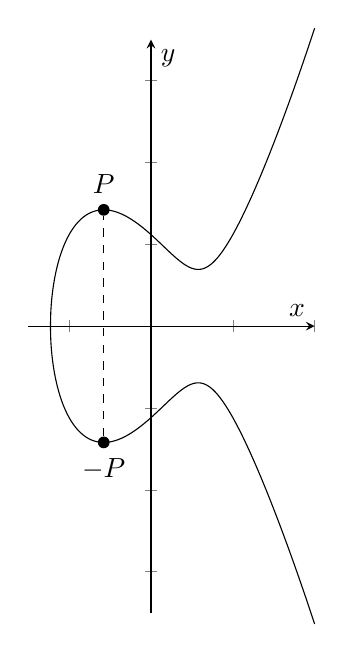
\begin{tikzpicture}
    \begin{axis}[
        xmin=-3,
        xmax=4,
        ymin=-7,
        ymax=7,
        xlabel={$x$},
        ylabel={$y$},
        scale only axis,
        axis lines=middle,
        % set the minimum value to the minimum x value
        domain=-2.456678:4,      % <-- works for pdfLaTeX and LuaLaTeX
        samples=1000,
        smooth,
        % to avoid that the "plot node" is clipped (partially)
        clip=false,
        % use same unit vectors on the axis
        axis equal image=true,
        xticklabels={,,},
        yticklabels={,,}
    ]
        \addplot [black] {sqrt(x^3-4*x+5)};
        \addplot [black] {-sqrt(x^3 - 4*x + 5)};
        
         % Some math constant macros
        \pgfmathsetmacro\localmaximum{-2/sqrt(3)}       
       	% add nodes to the points and the corresponding labels
       	\node [label={$P$}, circle,fill,inner sep=1.5pt] (P) at (\localmaximum, 2.842) {};
		\node [label=below:{$-P$}, circle,fill,inner sep=1.5pt] (-P) at (\localmaximum, -2.842) {};
       	\draw [black, dashed] (-P) -- (P);
    \end{axis}
\end{tikzpicture}
		\label{subfig: elliptic_curve_inv}
	}
	\captionof{figure}{Geometric interpretation of point addition, doubling and inversion when considering an elliptic curve over the real numbers \cite{paar2009understanding}.}
	\label{fig: elliptic curve operations geometric interpretation}
\end{figure}
%
If we work with elliptic curves, it is important to know the order of the group.
This order plays a key role in the hardness of the discrete log problem (DLP) that can be constructed with elliptic curves.
Hasse's theorem states that the number of points of an elliptic curve modulo a prime $p$ is roughly in the range of the prime $p$.
Each point on the curve also has an order.
The order of a point $P$ is the smallest positive integer $n$ such that:
%
\begin{align*}
[n]P = \overbrace{P \oplus \ldots \oplus P}^{n \text{ times}} = \mathcal{O}
\end{align*}
%
Some points never add up to $\mathcal{O}$, which gives them an infinite order.
The order of the neutral element is 1.
In cryptography, elliptic curves are treated on a given finite field, for example $K = \mathbb{F}_{p}$, with $p$ being a sufficiently large prime number.
Points on an elliptic curve together with the neutral element $\mathcal{O}$ have cyclic subgroups.
To make all points on the elliptic curve form a cyclic group, certain conditions have to be met.
$K = \mathbb{F}_{p}$ with $p > 3$ must hold.
In addition, the discriminant of the curve has to be non-zero (as mentioned earlier).
There are also other mathematical properties leading to cryptographic weaknesses that need to be ruled out.
Due to the complexity of constructing save curves, we often make use of standardized curves in practice.
Because we know the basic math behind elliptic curves, we can now construct a DLP over these curves \cite{paar2009understanding}:
%
\begin{definition}[Elliptic Curve Discrete Logarithm Problem (ECDLP)]
Given an elliptic curve $E$, a primitive element (also called a generator) $P$ and another element $T$. 
The discrete logarithm problem is finding the integer $d$, with $1 \le d \le \#(E)$ (with $\#(E)$ being the number of points on the curve) such that:
%
\begin{align*}
\overbrace{P \oplus P \oplus \ldots \oplus P}^{d \text{ times}} = dP = T
\end{align*}
%
\end{definition}
%
In cryptosystems, the value of $d$ becomes the private key, while the public key is $T$, where $T=(x_t, y_t)$ is a point on the curve.

% !TeX spellcheck = en_US
% !TeX root = ../Tom_Sandmann-master_thesis
\section{Twisted Edwards curves} \label{sec: Twisted Edwards curves}
Edwards curves are a family of elliptic curves \cite{edwards2007normal}.
An Edwards curve over a field $K$ having a characteristic unequal to 2 is defined as follows:
%
\begin{align*}
x^2 + y^2 = 1 + dx^2 y^2
\end{align*}
%
with scalar $d \in K \setminus \{0, 1\}$.
A more general form which introduces additional parameters also belongs to this family of curves:
%
\begin{align*}
x^2 + y^2 = c^2(1 + dx^2 y^2)
\end{align*}
%
with $c, d \in K$ and $c \cdot d (1 - c^4 \cdot d) \neq 0$.
The value of $c$ however is often fixed at 1.
This is also assumed when we introduce the addition and subtraction formula's for Edwards curves.
Every Edwards curve is birationally equivalent to an elliptic curve in Weierstrass form.
% https://crypto.stackexchange.com/questions/43013/what-does-birational-equivalence-mean-in-a-cryptographic-context
When we have geometric objects like elliptic curves, we want to define what it means for these two objects to be ``the same''.
Given two curves $E_1$ and $E_2$, we say that they are ``the same'' when they are isomorphic. Given two mathematical objects, they are said to be isomorphic if there exists an isomorphism between them. An isomorphism is a structure-preserving map (also called a homomorphism) that has an inverse.
Besides this way of equating objects, we also have another way of equating them.
That is by stating they are ``almost the same''.
This is exactly what a birational equivalence can be used for.
Two curves $E_1$ and $E_2$ are birationally equivalent when there exists a map $\phi : E_1 \to E_2$ between the two curves which is defined at every point of $E_1$ except for a small subset.
In addition, there is also an inverse map $\phi^{-1} : E_2 \to E_1$ which is again defined at every point of $E_2$ except for a small subset.
% https://crypto.stackexchange.com/questions/27842/edwards-montgomery-ecc-with-weierstrass-implementation
Before we show the birational equivalence between an Edwards curves and an elliptic curve in Weierstrass form, we first introduce a generalization of Edwards curves, which are called twisted Edwards curves \cite{bern2008twisted}.
Each twisted Edwards curve is a twist of an Edwards curve.
If we have an elliptic curve $E$ over a field $K$, then there exists a so-called quadratic twist, which is another elliptic curve which is isomorphic to $E$ (over an algebraic closure of $K$).
Given a field $K$ with $\operatorname{char}(k) \neq 2$, we define a twisted Edwards curve with the following equation:
%
\begin{align*}
E_{E,a,d} : ax^2 + y^2 = 1 + dx^2y^2
\end{align*}
%
with $a,d \in K \setminus \{0\}$ and $a \neq b$.
Note that a `normal' Edwards curve is just a specific instance of a twisted Edwards curve (it fixes $a = 1$). 
It can be shown that every twisted Edwards curve is birationally equivalent to an elliptic curve in Montgomery form and vice versa \cite{bern2008twisted}.
In addition, every Montgomery curve is also birationally equivalent to an elliptic curve in Weierstrass form.
A Montgomery curve is also a form of an elliptic curve. 
A Montgomery curve over a field $K$ is defined as follows:
%
\begin{align*}
E_{M, A, B} : Bv^2 = u^3 + Au^2 + u
\end{align*}
%
with $A, B \in K$ and $B(A^2 - 4) \neq 4$.
As with the curves we have described previously, this curve is generally considered over a finite field $K$ with characteristic unequal to 2 and $A \in K \setminus \{-2, 2\}$ and $B \in K \setminus \{0\}$.
The corresponding birational maps between these three curves are defined as follows \cite{bern2008twisted}:
%
\begin{theorem}[Birational equivalence between Montgomery curves and twisted Edwards curves]
	Let $E_{E,a,d}$ and $E_{M,A, B}$ be elliptic curves in twisted Edwards form and Montgomery form respectively (with their corresponding definitions as introduced earlier).
	A twisted Edwards curve $E_{E,a,d}$ is birationally equivalent to the Montgomery curve $E_{M, A, B}$, where:
	%
	\begin{align*}
		A = \frac{2(a + d)}{(a - d)} \text{, and } B = \frac{4}{a - d}
	\end{align*}
	%
	The birational equivalence from $E_{E_{a,d}}$ to $E_{M_{A, B}}$ is given by the following map:
	%
	\begin{align*}
	& \psi : E_{E,a,d} \to E_{M,A,B} \\
	& (x, y) \mapsto (u,v) = \left( \frac{1 + y}{1 - y}, \frac{1 + y}{(1 - y)x}\right)
	\end{align*}
	%
	with the following inverse:
	%
	\begin{align*}
	& \psi^{-1} : E_{M,A, B} \to E_{E,a,d} \\
	&  (u,v) \mapsto \left(\frac{u}{v}, \frac{u - 1}{u + 1} \right), a = \frac{A + 2}{B}, d = \frac{A - 2}{B}
	\end{align*}
	%
	The map $\psi$ is not defined at the points $v = 0$ or $u + 1 = 0$ of $E_{M,A,B}$.
\end{theorem}
%
\begin{theorem}[Birational equivalence between Montgomery curves and Weierstrass curves]
	Let $E_{M,A,B}$ and $E_{a,b}$ be elliptic curves in Montgomery form and in short Weierstrass form respectively (with their corresponding definitions as introduced earlier).
	The birational equivalence from $E_{M,A,B}$ to $E_{a,b}$ is given by the following map:
	%
	\begin{align*}
	& \psi : E_{M,A,B} \to E_{a, b} \\
	& (x, y) \mapsto (t,v) = \left( \frac{x}{B} + \frac{A}{B}, \frac{y}{B} \right), a = \frac{3 - A^2}{3B^2}, b = \frac{2A^3 - 9A}{27B^3}
	\end{align*}
	%
	For the inverse map to be valid, a couple of conditions have to be satisfied.
	Assume we have an elliptic curve $E_{a,b}$ over a base field $\mathbb{F}$, which is a curve over a field that is contained in all other fields (when working over a collection of fields).
	We can transform $E_{a,b}$ to its corresponding Montgomery form if and only if the order of $E_{a,b}$ is divisible by four and if the following conditions are satisfied \cite{okeya2000elliptic}:
	%
	\begin{itemize}
		\item The equation $x^3 + ax + b$ in $E_{a,b} : y^2 = x^3 + ax + b$ has at least one root in the finite field $\mathbb{F}_p$ of order $p$ with $p \ge 5$ being a prime;
		
		\item The number $3\alpha^2 + a$ is a quadratic residue in $\mathbb{F}_p$ (i.e. there exists an integer $x$ such that  $x^2 \equiv 3\alpha^2 + a \pmod{p}$), with $\alpha$ being the root of the equation $x^3 + ax + b = 0$ in $\mathbb{F}_p$.
	\end{itemize}
	%
	If these conditions are satisfied, then we have the following inverse of the map:
	%
	\begin{align*}
	& \psi^{-1} : E_{a, b} \to E_{M,A,B}  \\
	&  (t,v) \mapsto (s(t - \alpha), sv), A = 3 \alpha s, B = s
	\end{align*}
	%
	with $s = \left( \sqrt{3 \alpha^2 + a} \right)^{-1}$.
\end{theorem}
%
Thus, points on twisted Edwards curves can (under certain conditions) also be represented as points on Weierstrass curves. 
By choosing an appropriate point to serve as the neutral element, every twisted Edwards curve therefore admits an algebraic group law. We can now define the doubling and addition formulas for twisted Edwards curves.
Let $P=(x_1, y_1)$ and $Q=(x_2, y_2)$ be points on a twisted Edwards curve $E_{E,a,d}$.
The addition of the points $P$ and $Q$ on $E_{E.a,d}$ is defined as follows:
%
\begin{align*}
P + Q &= (x_1, y_1) + (x_2, y_2) = (x_3, y_3) \\
x_3 &= \frac{x_1 y_2 + y_1 x_2}{1 + d x_1 x_2 y_1 y_2} \\
y_3 &= \frac{y_1 y_2 - a x_1 x_2}{1 - d x_1 x_2 y_1 y_2}
\end{align*}
%
The doubling of a point $P=(x_1, y_1)$ uses exactly the formula as for addition, but can be simplified as follows:
%
\begin{align*}
2P &= (x_1, y_1) + (x_1, y_1) = (x_3, y_3) \\
x_3 &= \frac{x_1 y_1 + y_1 x_1}{1 + d x_1 x_1 y_1 y_1} = \frac{2 x_1 y_1}{ax_1^2 + y_1^2} \\
y_3 &= \frac{y_1 y_1 - a x_1 x_1}{1 - d x_1 x_1 y_1 y_1} = \frac{y_1^2 - ax_1^2}{2 - ax_1^2 - y_1^2}
\end{align*}
%
The neutral element is $\mathcal{O} = (0, 1)$.
The inverse of a point $(x_1, y_1)$ is defined as $(-x_1, y_1)$.
As mentioned before, we used the same formulas for both addition and doubling, but we were able to simplify these formulas in the doubling case.
In addition, the addition formula is also complete, which means that there are no exceptional cases when applying this formula.
% !TeX spellcheck = en_US
% !TeX root = ../Tom_Sandmann-master_thesis
\section{Alternative representations for fast computations} \label{sec: Alternative representations for fast computations}
% https://en.wikipedia.org/wiki/Affine_space#Informal_description
% https://www.cosic.esat.kuleuven.be/bcrypt/lecture%20slides/wouter.pdf
% https://math.stackexchange.com/questions/2331544/difference-between-affine-and-projective-elliptic-curve
% https://perso.univ-rennes1.fr/christophe.ritzenthaler/cours/elliptic-curve-course.pdf
% https://en.wikipedia.org/wiki/Linear_map#Definition_and_first_consequences
By changing the point representation of the points on the Edwards curve, we can increase the computation speed of the operations on these points.
In our definition of an elliptic curve in Weierstrass form, we defined an algebraic affine curve which is a curve in affine space.
In the following subsections, we introduce the concepts of affine and projective space, and describe how they are related.

\subsection{Affine space}
Informally, an affine space is what is left of a vector space once we have forgotten which point is the origin. Instead, we add translations to the linear maps over the vector space.
% https://math.stackexchange.com/questions/1303351/need-help-understanding-wikis-informal-description-of-an-affine-space
A simple explanation in the form of an analogy can be found on Wikipedia%
\footnote{\url{https://en.wikipedia.org/wiki/Affine_space}}.
Assume Alice and Bob want to add two vectors $\vec{a}$ and $\vec{b}$ (which are vectors measured from Alice's origin). 
However, both Alice and Bob disagree about which point is the origin. Alice knows that a certain point is the actual origin, but Bob believes that this is another point, which we call $p$.
Note that both Alice and Bob agree on which \textit{points} are $a$ and $b$, but disagree about the correspondence between \textit{points} and \textit{vectors}.
To add the vectors, Bob draws an arrow from point $p$ to point $a$ and another arrow from point $p$ to point $b$, thus completing the parallelogram for vector addition and finding the resulting point which Bob believes is $\vec{a} + \vec{b}$.
Alice however knows that Bob actually computed the following:
%
\begin{align*}
p + (\vec{a}- p) + (\vec{b} - p)
\end{align*}
%
Note that the point-from-vector subtraction seems odd at first sight.
However, if we combine it with the addition notation $p + \vec{v}$, we can interpret it as follows: ``the result point after applying the transformation represented by vector $\vec{v}$ to point $p$''.
Similarly, Alice and Bob can evaluate any linear combination of $\vec{a}$ and $\vec{b}$ or any finite set of vectors with generally different answers.
If the sum of coefficients in the linear combination adds up to 1, then both Alice and Bob will end up with the same answer. So if Alice evaluates the following expression:
%
\begin{align*}
\lambda \vec{a} + (1 - \lambda) \vec{b}
\end{align*}
%
then Bob similarly will evaluate
%
\begin{align*}
p + \lambda (\vec{a} - p) + (1-\lambda)(\vec{b} - p) &= p + \lambda \vec{a} - \lambda p + \vec{b} - p - \lambda \vec{b} + \lambda p \\
&= \cancel{p - p + \lambda p - \lambda p} + \lambda \vec{a} + \vec{b} - \lambda \vec{b} \\
&= \lambda \vec{a} + (1 - \lambda) \vec{b}
\end{align*}
%
Thus Alice and Bob describe the same point with the same linear combination for all coefficients $\lambda + (1 - \lambda) = 1$, despite making use of different origins.
Only Alice knows the ``linear structure'' of the result, but they both know the ``affine structure'' which is the linear combination of vectors in which the sum of the coefficients adds up to 1 (such a linear combination is also called an affine combination).
A set which has an affine structure is called an affine space.

% https://crypto.stackexchange.com/questions/40947/what-is-the-projective-space
% https://mathoverflow.net/questions/87847/explaining-the-concept-of-projective-space-notes-for-students
\subsection{Projective space}
Besides having affine coordinates in affine space, we can also have projective coordinates in projective space.
We often make use of the Cartesian coordinate system, which is a coordinate system that specifies each point in a plane uniquely by a pair of numerical coordinates. These points are described by signed distances from two fixed perpendicular lines which are called the axes of the system. The origin is the ordered pair $(0, 0)$, which is the point where both axes intersect. Points can also be described in $n$-dimensional Euclidean space, for any dimension $n$.
Similarly how Cartesian coordinates are used in Euclidean geometry, \textit{projective coordinates} or homogeneous coordinates are used in projective geometry. 
Affine spaces are subspaces of projective spaces.
We can obtain an affine plane from any projective plane by removing a line and all the points on it.
The other way around, we can also obtain a projective plane from an affine plane by adding a line at infinity.
An advantage of projective coordinates is the fact that formulas involving these kind of coordinate are often simpler and more symmetric than their corresponding Cartesian formulas.
In addition, projective coordinates can be used to represent points at infinity, although the coordinates to represent these points are finite themselves.
Assume we have a point $(x, y)$ on the Euclidean plane.
The triple $(xZ, yZ, Z)$, with $Z \in \mathbb{R} \setminus \{0\}$ is called a \textit{set of projective coordinates} for the point.
If we multiply this triple by a non-zero scalar we get a new set of projective coordinates for the same point. 
For example, the Cartesian point $(1, 2)$ can be represented in projective coordinates as $(1, 2, 1)$ but also as  $(2, 4, 2)$. 
Thus a single point can be represented by an infinite number of projective coordinates, which is not possible using Cartesian coordinates.

To summarize, any point in the projective plane is represented by a triple $(X, Y, Z)$ which are called the projective coordinates of the point, with $X, Y$ and $Z$ being nonzero.
If the value of $Z$ is unequal to zero, the point represented is the point $(X/Z, Y/Z)$ in the Euclidean plane. If value of $Z$ is zero however, the point represented is the point at infinity. The origin is represented by the triple $(0, 0, 1)$, and the triple $(0, 0, 0)$ is removed and does not represent any point. So far, we assumed the points in projective 2-space.
In general, points in projective $n$-space are represented by $(n + 1)$-tuples. 

\vspace{5mm} \noindent
%
Now we have become familiar with projective coordinates, its time to introduce some alternative representations in which a point on a twisted Edwards curve can be represented.
The formula for point addition on twisted Edwards curves (which can also be used for point doubling) as shown in \Cref{sec: Twisted Edwards curves} has a cost of $10\bm{\mathrm{M}}$ and $1\bm{\mathrm{S}}$ when the curve parameters are chosen properly \cite{bernstein2007inverted}.
The cost of a formula is denoted with $\bm{\mathrm{M}}$, $\bm{\mathrm{S}}$, $\bm{\mathrm{D}}$ and $\bm{\mathrm{A}}$ which respectively denote the cost of one multiplication, one squaring, one doubling and one addition. 
In the upcoming sections, we provide formulas that are \emph{strongly unified}.
A formula is strongly unified when it works for both the addition and doubling cases without any change.
A related concept is \emph{completeness}, which means that a formula can handle any input.
This property is discussed per representation.
%
% Strongly Unified -> https://en.wikipedia.org/wiki/Edwards_curve
% Meaning: "One of the attractive feature of the Edwards Addition law is that it is strongly unified i.e. it can also be used to double a point, simplifying protection against side-channel attack."
% Extended -> strongly unified: http://hyperelliptic.org/EFD/g1p/auto-twisted-extended.html#addition-add-2008-hwcd-2
% Complete -> These unified formulae are derived from the addition formulae (1). We deduce from [5] and [1] that these formulae are also complete when d is not a square in K and a is a square in K
\subsection{Extended twisted Edwards coordinates} \label{subsec: Extended twisted Edwards coordinates}
A point $(x, y, t)$ with $t=x \cdot y$ on the twisted Edwards curve $E_{E,a,d}$ can be represented as the 4-tuple $(X:Y:T:Z)$ that satisfies the following equations \cite{hisil2008twisted}:
%
\begin{align*}
x &= X/Z \\
y &= Y/Z \\
t &= T/Z
\end{align*}
%
We can pass to the projective representation by making use of the following map: $(x, y, t) \mapsto (x:y:t:1)$.
The identity element is now represented by $(0: 1: 0: 1)$, and the negative of $(X:Y:T:Z)$ is defined as $(-X:Y:-T:Z)$.
The coordinates of the point $(X:Y:Z:T)$ are called the \emph{extended twisted Edwards coordinates}.
Addition is defined as $(X_1 : Y_1 : T_1 : Z_1) + (X_2 : Y_2 : T_2 : Z_2) = (X_3 : Y_3 : T_3 : Z_3)$.
The explicit unified formula for addition can be seen in \Cref{table: extended twisted Edwards explicit formulas alternative representations}, and is complete if $d$ is a non-square in $K$ and $a$ a square in $K$ \cite{hisil2008twisted}.
Despite the additional overhead of computing the newly introduced auxiliary variable $t$, this new system allows for faster point addition \cite{hisil2008twisted}, as it saves $1\bm{\mathrm{M}}$.

%Inverted -> strongly unified: http://hyperelliptic.org/EFD/g1p/auto-twisted-inverted.html#addition-add-2008-bbjlp
\subsection{Inverted twisted Edwards coordinates}
In \cite{bernstein2007inverted}, another representation called \emph{Inverted twisted Edwards coordinates} is introduced for $E_{E,a,d}$ with  $a = 1$. They use the coordinates $(X_1 : Y_1 : Z_1)$ where
%
\begin{align*}
\left( X_1^2 + Y_1^2 \right) Z_1^2 = X_1^2 Y_1^2 + dZ_1^4
\end{align*}
%
with $X_1 Y_1 Z_1 \neq 0$.
A point on the twisted Edwards curve $E_{E,a,d}$ (with $a = 1$) is now represented as $(Z/X, Z/Y)$.
The explicit formulas for addition can be seen in \Cref{table: extended twisted Edwards explicit formulas alternative representations}.
Addition is defined as $(X_1 : Y_1 : Z_1) + (X_2 : Y_2 : Z_2) = (X_3 : Y_3 :  Z_3)$.
One of the advantages of this representation is that they save one multiplication ($1\bm{\mathrm{M}}$) for each addition, without slowing down doubling or tripling.
The addition formula is not complete. 
The requirement $X_1 Y_1 Z_1 \neq 0$ implies that points on the Edwards curve that satisfy $x_1 y_1 = 0$ cannot be represented in inverted Edwards coordinated. 
As we know, there are four points that satisfy this requirement: the neutral element $(0, 1)$, the point $(0, -1)$ of order 2 and the points $(\pm 1, 0)$ of order 4.
To be able to handle these case as inputs or outputs, special routines need to used (which we do not describe here).


%Projective -> strongly unified: https://hyperelliptic.org/EFD/g1p/auto-twisted-projective.html#addition-add-2008-bbjlp
\subsection{Projective twisted Edwards coordinates}
Another way to avoid costly inversions is to work with projective twisted Edwards curves \cite{bern2008twisted}.
This curve has the following equation:
%
\begin{align*}
	(aX^2 + Y^2) Z^2 = Z^4 + dX^2Y^2
\end{align*}
%
with $Z_1 \neq 0$ and the projective point $(X_1 : Y_1 : Z_1)$.
This projective point represents the affine point $(X_1 / Z_1, Y_1 / Z_1)$ on  $E_{E, a, d}$.  The explicit formulas for addition and doubling can be seen in \Cref{table: extended twisted Edwards explicit formulas alternative representations}.
Addition is defined as $(X_1 : Y_1 : Z_1) + (X_2 : Y_2 : Z_2) = (X_3 : Y_3 :  Z_3)$. The formula shown \Cref{table: extended twisted Edwards explicit formulas alternative representations} for the projective case has a cost of $10\bm{\mathrm{M}}$ (which is exactly the same as the original Edwards formula) and is complete.
However, for certain values of $Z_1$ and $Z_2$, the cost of this formula can be greatly reduced: assuming $Z_1 = 1$ and $Z_2 = 1$, there exist an addition formula using this representation which only requires $6\bm{\mathrm{M}}$.
%
\begin{table}
	\centering
	\begin{adjustbox}{width=\textwidth}
		\begin{tabular}{lll}
			\toprule
			\textbf{Extended} & \textbf{Inverted} & \textbf{Projective} \\
			\midrule 
			{$\!\begin{aligned}
				A &= X_1 \cdot X_2 \\
				B &= Y_1 \cdot Y_2 \\
				C &= T_1 \cdot dT_2 \\
				D &= Z_1 \cdot Z_2 \\
				E &= (X_1+Y_1) \cdot (X_2+Y_2)-A-B \\
				F &= D-C \\
				G &= D+C \\
				H &= B-aA \\
				X_3 &= E \cdot F \\
				Y_3 &= G \cdot H \\
				T_3 &= E \cdot H \\
				Z_3 &= F \cdot G \\
				\end{aligned}$}
			& 
			{$\!\begin{aligned}
				A &= Z_1 \cdot Z_2 \\
				B &= d A_2 \\
				C &= X_1 \cdot X_2 \\
				D &= Y_1 \cdot Y_2 \\
				E &= C \cdot D \\
				H &= C-a D \\
				I &= (X_1+Y_1) \cdot (X_2+Y_2)-C-D \\
				X_3 &= (E+B) \cdot H \\
				Y_3 &= (E-B) \cdot I \\
				Z_3 &= A \cdot H \cdot I \\
				\end{aligned}$}
			&
			{$\!\begin{aligned}
				A &= Z_1 \cdot Z_2 \\
				B &= A_2 \\
				C &= X_1 \cdot X_2 \\
				D &= Y_1 \cdot Y_2 \\
				E &= dC \cdot D \\
				F &= B-E \\
				G &= B+E \\
				X_3 &= A \cdot F ((X_1+Y_1) \cdot (X_2+Y_2)-C-D ) \\
				Y_3 &= A \cdot G (D-aC) \\
				Z_3 &= F \cdot G \\
				\end{aligned}$}
			\\
			\bottomrule
		\end{tabular}
	\end{adjustbox}
	\captionof{table}{Explicit strongly unified addition formulas for extended, inverted and projective twisted Edwards curve coordinates \cite{hisil2008twisted}.}
	\label{table: extended twisted Edwards explicit formulas alternative representations}
\end{table}
%
% !TeX spellcheck = en_US
% !TeX root = ../Tom_Sandmann-master_thesis
\section{Efficient scalar multiplication}
Gallant--Lambert--Vanstone (GLV) method is a way of speeding up the computation of scalar multiplications on some elliptic curves defined over fields with a large prime characteristic.
Assume we have an elliptic curve of prime order $n$ with a point $P$.
By making use of the GLV method, we try to find a decomposition of the scalar multiplication $[k]P$ for $k \in \{1, \ldots, n\}$ into, for example, two scalar multiplications $[k]P = [u]P + [v]Q$.
This is a multi-exponentiation.
In general, a multi-exponentiation has the following form:
%
\begin{align*}
\sum_{i = 0}^{i < m} k_i P_i
\end{align*}
%
In the example we gave, the value of $m$ would be 2.
By rewriting this scalar multiplication, the new scalars $u, v$ only have half of the bitlength compared to the original bitlenght of the scalar $k$.
Such a scalar multiplication which involves two different points and two different scalars is computed by a \emph{double point multiplication} algorithm.
One obvious way to compute a double point multiplication is to perform two single-point multiplications. However, multiple algorithms exists that can compute $[u]P + [v]Q$ simultaneously and therefore more efficiently.
One of these algorithms is called the Straus-Shamir trick, which is an algorithm that can be used for simultaneous point multiplication.
The trick is in building one sequence of intermediate results that directly converge to the value of $[u]P + [v]Q$ in one execution of a Double-and-Add algorithm (which would be the traditional way of computing the scalar multiplication).
%https://books.google.nl/books?id=EQXnAwAAQBAJ&pg=PA174&lpg=PA174&dq=straus-shamir+trick+with&source=bl&ots=zaRlEXEtqD&sig=-0HGrNiuvnQ7qRNiu5Ac5_5Rgsg&hl=en&sa=X&ved=0ahUKEwjnvvfLmsHaAhXL-6QKHZ3pCYgQ6AEIXjAI#v=onepage&q=straus-shamir%20trick%20with&f=false
%http://cacr.uwaterloo.ca/hac/about/chap14.pdf
The algorithm can be seen in \Cref{algo: Straus-Shamir Trick} , where $\mathcal{S}$ is some set of integers containing 0 and 1 (as presented in \cite{moller2002improved}) and $\mathcal{E}$ an elliptic curve.
%
\begin{algorithm}
	\algorithmicrequire  $u = \sum_{i = 0}^{\ell - 1} u_i 2^i, v = \sum_{i = 0}^{\ell - 1} v_i 2^i, (u_{\ell - 1}, v_{\ell - 1}) \neq (0, 0), (u_i, v_i) \in \mathcal{S}^2, (P, Q) \in \mathcal{E}^2, P \neq \pm Q$.\\
	\algorithmicensure $R = [u] P + [v] Q$.
	%	
	\begin{algorithmic}[1]
		\State Precompute $W_{i, j} = [i]P + [j]Q, \forall(i, j) \in \mathcal{S} \setminus \{(0, 0)\}$
		\State Initialize $W_{u_{\ell -1}, v_{\ell - 1}}$
		\For {$i = \ell - 2$ \textbf{downto} $0$}
			\State $R = [2]R$
			\If{$(u_i, v_i) \neq (0, 0)$}
				\State $R = R + W_{u_i, v_i}$
			\EndIf
		\EndFor
	\end{algorithmic}
	%
	\captionof{algorithm}{Double Scalar Multiplication using the Straus-Shamir Trick \cite{rondepierre2013revisiting}.}
	\label{algo: Straus-Shamir Trick}
\end{algorithm}
%
The Straus-Shamir trick is actually a special case of Straus' algorithm, in which the window size is set to 1.
This trick reduces the number of doublings by half.
To further increase the performance, we can make use of signed digit representations and windowing.
By making use of these methods, we can increase the number of null digits of the scalar, which increases the performance by reducing the number of additions.
These methods require the scalar to be transformed to another representation, which is called \emph{scalar recoding}.
We discuss other methods of performing efficient scalar multiplications in the upcoming subsections.

\subsection{Comb method} \label{subsec: Comb method}
The comb method is a way to perform scalar multiplication.
The method assumes that the scalar $k$ is represented by a matrix of $w$ rows and $d$ columns.
During the scalar multiplication, $k$ is being processed columwise. 
Initially, the binary representation of $k$ is first padded on the left with $dw - t$ zeros, such that its length is $dw$.
$k$ is now split up into $w$-bit strings $K$ with each of these string having a length of $d$, such that:
%
\begin{equation*}
k = K^{w-1} \Vert \dots \Vert  K^{1} \Vert K^0
\end{equation*}
%
with $\Vert$ denoting the bitwise concatenation operator.
The bit strings $K^j$ are now written as rows of an \emph{exponent array} \cite{hankerson2006guide}:
%
\begin{equation*}
%
\begin{bmatrix}
		K^0 \\
		\vdots \\
		K^{w'} \\
		\vdots \\
		K^{w - 1}
\end{bmatrix}
%
=
%
\begin{bmatrix}
k_{d-1}^0 & \dots & k_0^0 \\
\vdots & & \vdots \\
K_{d-1}^{w'} & \dots & K_0^{w'} \\
\vdots & & \vdots \\
K_{d-1}^{w-1} & \dots & K_0^{w - 1}
\end{bmatrix}
%
=
%
\begin{bmatrix}
k_{d-1} & \dots & k_0 \\
\vdots & & \vdots \\
K_{(w'+1)d-1} & \dots & K_{w'd} \\
\vdots & & \vdots \\
K_{wd-1} & \dots & K_{(w-1)d}
\end{bmatrix}
\end{equation*}
%
The columns of this exponent array will then be processed one at a time from left to right during the scalar multiplication.
To speed up the computation of the scalar multiplication, the following points are precomputed \cite{hankerson2006guide}:
%
\begin{align*}
\left[ a_{w - 1}, \ldots, a_2, a_1, a_0 \right]P = a_{w-1} 2^{(w-1)d} P + \ldots + a_2 2^{2d} P + a_1 2^ d P + a_0 P
\end{align*}
%
This precomputation is done for all possible bit strings $(a_{w - 1}, \ldots, a_1, a_0)$.
The algorithm itself can be seen in \Cref{algo: Fixed-base comb method for point multiplication}.
%
\begin{algorithm}
	\algorithmicrequire Scalar $k = (k_{t-1}, \ldots, k_1, k_0)_2$, window width $w$, bit string size $d = \lceil t / w\rceil$ and $P \in E(\mathbb{F}_p)$.
	\algorithmicensure $R = [k]P$.
	%	
	\begin{algorithmic}[1]
		\Statex \textbf{Precomputation}
		\State Compute $[ a_{w - 1}, \ldots, a_2, a_1, a_0 ]P$ for all bit strings  $(a_{w - 1}, \ldots, a_1, a_0)$ with length $w$
		\State Write $k = K^{w-1} \Vert \dots \Vert  K^{1} \Vert K^0$ and add padding on the left if necessary. Each $K^j$ is a bit string of length $d$. With $K_i^j$ we denote the $i$-th bit of the bit string $K^j$.
			\State $R \gets \infty$
		\For {$i = d - 1$ \textbf{downto} $0$}
			\State $R \gets 2R$
			\State $R \gets R + \left[ K_i^{w-1}, \ldots, K_i^1, K_i^0 \right] P$
		\EndFor
		\State \textbf{Return} $Q$
	\end{algorithmic}
	%	
	\captionof{algorithm}{Fixed-base comb method for point multiplication \cite{hankerson2006guide}.}
	\label{algo: Fixed-base comb method for point multiplication}
\end{algorithm}
%

% NAF: https://crypto.stackexchange.com/a/25229
\subsection{Interleaving}
Another way of performing scalar multiplication is by making use of interleaving.
As we have seen with the Straus-Shamir trick, the precomputed values were obtained by making use of two points. 
When each precomputed value only involves one point, the associated method of multiple point multiplication is also known as \emph{interleaving}.
An example of such a method is an interleaving algorithm which makes use of the \textbf{non-adjacent form (NAF)} of a number.
The NAF of a number is a unique signed-digit representation, which means that non-zero values cannot be adjacent.
The integer $7$ in NAF would be represented as follows: $(1~0~0~\bar{1})$, where $\bar{1} = - 1$.
There exist different algorithms to convert a number to NAF, one of which is introduced in \cite{hankerson2006guide}.
If we want to transform an integer $k$ to NAF, this algorithm will repeatedly divide $k$ by 2. 
Remainders of $0$ or $\pm 1$ are allowed, but if $k$ is odd, then the remainder $r \in \{-1, 1\}$ is chosen in such a way that the quotient $(k - r) / 2$ is even.
This makes sure that the next NAF digit is 0.
The corresponding algorithm can be seen in \Cref{algo: compute NAF}.
% Two algorithms side by side, see https://tex.stackexchange.com/questions/418185/putting-two-algorithms-side-by-side-with-reasonable-margin
\begin{figure}
%
	\begin{minipage}[t]{7.0cm}%
		\vspace{2pt}
		\begin{algorithm}[H]
			\algorithmicrequire A positive integer $k$.\\
			\algorithmicensure $\text{NAF}(k)$.
			%	
			\begin{algorithmic}
				\State $i \gets 0$
				\While{$k \ge 1$}
				\If{$k$ is odd}
				\State $k_i \gets 2 - (k \pmod{4})$ \label{lst: Interleaving with NAFs: line change for w-width NAF}
				\State $k \gets k - k_i$
				\Else
				\State $k_i \gets 0$
				\EndIf
				\State $k \gets k / 2$
				\State $i \gets i + 1$
				\EndWhile
				\State \textbf{Return} $(k_{i - 1}, k_{i - 2}, \ldots, k_1, k_0)$
			\end{algorithmic}
			%
			\captionof{algorithm}{Computing the NAF of a positive integer \cite{hankerson2006guide}.}
			\label{algo: compute NAF}
		\end{algorithm}
		% @see Guide to Elliptic Curve Cryptography
	\end{minipage}%
	%
	\hfill%
	%
	\begin{minipage}[t]{7.0cm}%
		\vspace{2pt}
		\begin{algorithm}[H]
			\algorithmicrequire A positive integer $k$.\\
			\algorithmicensure $\text{NAF}_w(k)$.
			%	
			\begin{algorithmic}
				\State $i \gets 0$
				\While{$k \ge 1$}
				\If{$k$ is odd}
				\State $k_i \gets k \operatorname{mods}{2^w}$
				\State $k \gets k - k_i$
				\Else
				\State $k_i \gets 0$
				\EndIf
				\State $k \gets k / 2$
				\State $i \gets i + 1$
				\EndWhile
				\State \textbf{Return} $(k_{i - 1}, k_{i - 2}, \ldots, k_1, k_0)$
			\end{algorithmic}
			%
			\captionof{algorithm}{Computing the width-$w$ NAF of a positive integer \cite{hankerson2006guide}.}
			\label{algo: compute NAF-w}
		\end{algorithm}
		% @see Guide to Elliptic Curve Cryptography
	\end{minipage}%
	%
\end{figure}
An interleaving method for computing $\sum_{j = 1}^{v} k^j P_j$ can be seen in \Cref{algo: interleaving with NAFs}.
%
\begin{algorithm}
	\algorithmicrequire  $v$, a set of integers $k^j$, widths $w_j$ and points $P_j$, with $1 \le j \le v$.\\
	\algorithmicensure $\sum_{j = 1}^{v} k^j P_j$.
	%
	\begin{algorithmic}[1]
		\State Compute $iP_j$ for $i \in \{1, 3 , \ldots, w^{w_j - 1} - 1\}$ for $1 \le j \le v$
		\State Compute NAF$_{w_j} (k^j) = \sum_{i = 0}^{l_j - 1} k_i^j 2^i$ for $1 \le j \le v$
		\State $l \gets \text{max} \{l_j : 1 \le j \le v \}$ \Comment{$l_j$ denotes the length of NAF$_{w_j}(k^j)$}
		\State $k_i^j = 0$ for $l_j \le i < l, 1 \le j \le v$
		\State $R \gets \infty$
		\For{$i = l-1$ \textbf{downto} $0$}
			\State $R \gets 2R$
			\For{$j = 1$ \textbf{to} $v$}
				\If{$k_i^j \neq 0$}
					\If{$k_i^j > 0$}
						\State $R \gets R + k_i^j P_j$
					\Else
						\State $R \gets R - k_i^j P_j$
					\EndIf
				\EndIf	
			\EndFor
		\EndFor
		\State \textbf{Return} $R$
	\end{algorithmic}
	%
	\captionof{algorithm}{Interleaving with NAFs \cite{hankerson2006guide}.}
	\label{algo: interleaving with NAFs}
\end{algorithm}
%
The algorithm makes use of a window method which processes only a particular number of digits at a time.

If $w \ge 2$ is a positive integer, then a \emph{width}-$w$ \emph{NAF} of a positive integer $k$ is an expression $k = \sum_{i = 0}^{l - 1} k_i 2^i$ in which each nonzero coefficient $k_i$ is odd. 
In addition, $\abs{k_i} < 2^{w - 1}$ with $k_{l - 1} \neq 0$. 
At most one of any $w$ consecutive digits is nonzero. The length of the width-\emph{w} NAF is $l$. 
Computation of a $w$-width NAF requires a small change of \Cref{algo: compute NAF} at \Cref{lst: Interleaving with NAFs: line change for w-width NAF}. This can be seen in \Cref{algo: compute NAF-w}.
Instead of calculating $k_i \gets 2 - (k \pmod{4})$, the computation becomes $k_i \gets k \operatorname{mods}{2^w}$, where $ k \operatorname{mods}{2^w}$ denotes the integer $u$ which satisfies $u \equiv k \pmod{2^w}$ with $-2^{w-1} \le u < 2^{w - 1}$ \cite{hankerson2006guide}.

We now discuss the interleaving algorithm shown in \Cref{algo: interleaving with NAFs}.
We explain how this algorithm works in the case of double exponentiation (i.e. $v = 2$).
If we want to calculate $R = [k_0^j]P + [k_1^j] Q$, we first precompute $\{P, 3P, 5P, \ldots, [(2w - 1) / 2]P \}$ and $\{ Q, 3Q, 5Q, \ldots, [(2w - 1)] P \}$ for a choice of window size $w$. 
We then convert both $k_0^j$ and $k_1^j$ to width-$w$ NAF format. 
After initializing a point $R$ to the point-at-infinity, we scan the NAFs for $k_0^j$ and $k_1^j$ from left to right. 
While we process each bit, we double the value of $R$. 
As we are scanning the NAFs, we choose the subsections of the corresponding NAF to get the largest multiple of $P$ or $Q$.
This value is present in the tables we precomputed earlier.
We add this precomputed multiple of $P$ or $Q$ to $R$.
As the value of $w$ becomes bigger, more time is required for precomputation.
This also increases the amount of memory needed to store these precomputed tables. 
However, in the end this leads to less additions in the main double-and-add loop which increases the performance of the algorithm.

Multi-exponentiation as shown in the \emph{Interleaving with NAFs} algorithm can also be done by making use of a morphism (also called a homomorphism).
A morphism is a structure-preserving map from an mathematical structure to itself.
An endomorphism is a morphism from a mathematical object to itself.
An example of an endomorphism is the Frobenius endomorphism, which is a special endomorphism of commutative rings with prime characteristic $p$.
The Frobenius morphism maps every elements to its $p$-th power.
If we have commutative ring $R$ with prime characteristic $p$, the Frobenius endomorphism is defined as:
%
\begin{align*}
F(p) = r^p
\end{align*}
%
for all $r \in R$.
We can make use of homomorphisms in variable point multiplication.
Assume we want to calculate $[k]p = [u]P + [v]Q$, where $Q = \psi(P)$ and $\varphi$ being a homomorphism.
Again we have the precomputed table $\{P, 3P, 5P, \ldots, [(2w - 1) / 2]P \}$.
We can now easily compute the other table by applying $\psi$ to each of the elements in the table we already precomputed.
This speeds up the precomputation phase.
This approach is also adopted by {\fourq}, and is described in more detail in \Cref{chp: FourQ}.
